\chapter{Número, variable y función}

\section{Números reales. Representación de número reales por medio de puntos en el eje numérico}

    %--------------------Definición 1.1.
    \begin{tcolorbox}[colframe=white]
	\begin{def.}
	    El número racional puede expresarse como la razón $\dfrac{p}{q}$ de dos números enteros $p$ y $q$.\\\\
	    El número entero $p$ se puede considerar como la razón de dos números enteros $\dfrac{p}{1}$.\\
	\end{def.}
    \end{tcolorbox}
       
    %--------------------Definición 1.2.
    \begin{tcolorbox}[colframe = white]
	\begin{def.}
	    Los números en forma de fracciones decimales indefinidas no periódicas, se denominan números irracionales.\\
	\end{def.}
    \end{tcolorbox}

    \begin{tcolorbox}[colframe=white]
	\begin{def.}
	    Para cualquier par de números reales $x$ e $y$ existen una correlación, y sólo una, de las siguientes:
	    $$x<y, \qquad x=y, \qquad x>y$$
	\end{def.}
    \end{tcolorbox}

	%--------------------teorema 1.1
	\begin{teo}
	    Todo número irracional $\alpha$ se puede expresar con cualquier grado de precisión por medio de números racionales.\\\\
	    Demostración.-\; En efecto, siendo el número irracional $\alpha>0$, calculamos $\alpha$ con un error no mayor de $\dfrac{1}{n}$ (por ejemplo,, de $\dfrac{1}{10}, \dfrac{1}{100},$ etc.)\\
	    Cualquiera que sea el número $\alpha$, está comprendido entre dos números enteros consecutivos $N$ y $N+1$. Dividamos el segmento comprendido entre $N$ y $N+1$ en n partes, entonces el número $\alpha$ resulta comprendido entre los número racionales $N + \dfrac{m}{n}$ y $N + \dfrac{m+1}{n}$. Dado que la diferencia entre estos números es $\dfrac{1}{n}$, cada uno de ellos expresa $\alpha$ con un grado de precisión predeterminado: El primero por defecto y el segundo por exceso.\\\\
	\end{teo}

\section{Valor absoluto del número real}

    %--------------------definición 1.3.
    \begin{tcolorbox}[colframe=white]
	\begin{def.}
	    Un número real no negativo, que satisface las condiciones: $$|x|=x, \; si \; x\geq 0;$$ $$|x| = -x, \; si \; x<0$$ se llama valor absoluto (o módulo) de un número real $x$.\\ 
	\end{def.}
    \end{tcolorbox}

    %-------------------- propiedades de valor absoluto

    %propiedad 1.1.
    \begin{tcolorbox}[colframe=white]
	\begin{prop}	
	    El valor absoluto de la suma albegraica de varios números reales no es mayor que la suma de los valores absolutos de los sumandos:
	    $$|x+y| \leq |x| +|y|$$\\\\
	    Demostración.-\; Sea $x+y\geq 0$, entonces:
	    $$|x+y| = x+y \leq |x| + |y| $$ (ya que $x\leq |x|$ e $y\leq |y|$). \\
	    Supongamos ahora que $x+y<0$, entonces:
	    $$|x+y| = -/x+y) = (-x) + (-y) \leq |x| + |y|,$$ como se trataba de demostrar.\\\\
	\end{prop}
    \end{tcolorbox}

    %propiedad 1.2.
    \begin{tcolorbox}[colframe=white]
	\begin{prop}
	  El valor absoluto de la diferencia de dos números no es mejor que la diferencia de los valores absolutos del minuendo y sustraendo:
	  $$|x-y|\geq |x| - |y|$$\\\\
	  Demostración\; Supongamos que $x-y=x$. Entonces $x=y+z$, y según lo demostrado anteriormente, se tiene:
	  $$|x|=|y+z| \leq |y| + |z| = |z| + |x-y|,$$ de donde $$|x| - |y| \leq |x-y|,$$ como se trataba de demostrar.\\\\
	\end{prop}
    \end{tcolorbox}

    %propiedades 1.3.
    \begin{tcolorbox}[colframe=white]
	\begin{prop}	
	    El valor absoluto del producto es igual al producto de los valores absolutos de los factores: $$|xyz| = |x||y||z|.$$
	\end{prop}
    \end{tcolorbox}

    %propiedad 1.4.
    \begin{tcolorbox}[colframe=white]
	\begin{prop}
	    El valor absoluto del cociente es igual al cociente de dividir el valor absoluto del dividendo por el del divisor:
	    $$\left| \dfrac{x}{y} \right| = \dfrac{|x|}{|y|}.$$\\
	\end{prop}
    \end{tcolorbox}

\setcounter{section}{3}
\section{Campo de variación de la magnitud variable}

    %--------------------definición 1.4.
    \begin{tcolorbox}[colframe=white]
	\begin{def.}
	    El conjunto de todos los valores numéricos de la masgnitud variable se denomina campo de variación de la variable.\\
	\end{def.}
    \end{tcolorbox}

\section{Variable ordenada. Variable crecientes y decrecientes , variable acotada}

    %--------------------definición 1.5.
    \begin{tcolorbox}[colframe=white]
	\begin{def.}
	    La variable se denomina creciente, si cada valor posterior es mayor que el anterior. Por el contrario, si cada valor posterior es menor que el anterior, la variable se denomina decreciente.\\
	\end{def.}
    \end{tcolorbox}

    %--------------------definición 1.6.
    \begin{tcolorbox}[colframe=white]
	\begin{def.}
	    La variable $x$ se denomina magnitud acotada, si existe un número constante $M>0$ tal que, a partir de cierto valor, todos los posteriores satisfagan la condición. $$-M\leq x \leq M, \quad es \; decir, \quad |x|\leq M$$\\
	\end{def.}
    \end{tcolorbox}

\section{Función}

    %--------------------definición 1.7
    \begin{tcolorbox}[colframe=white]
	\begin{def.}
	    Si a cada valor de la variable $x$, perteneciente a cierto campo, le corresponde un sólo valor determinado de otra variable y, entonces ésta será función de $x$, y podemos escribir simbólicamente: $$y=f(x), \quad y = g(x), \quad etc.$$\\\\
	    La dependencia que existe entre las variables $x$ e $y$ se llaman funcional.\\
	\end{def.}
    \end{tcolorbox}

    %--------------------definición 1.8
    \begin{tcolorbox}[colframe=white]
	\begin{def.}
	    El conjunto de los valores de $x$ para los cuales se terminan los valores de la función $y$, en virtud de la ley $f(x)$, se llama \textbf{dominio de definición de la función}\\
	\end{def.}
    \end{tcolorbox}

    %--------------------definición 1.9
    \begin{tcolorbox}[colframe = white]
	\begin{def.}
	    La función $y=f(x)$ se llama creciente, cuando a un mayor valor del argumento $x$ corresponde un mayor valor de la función. De modo análogo se define la función decreciente.\\
	\end{def.}
    \end{tcolorbox}

\setcounter{section}{7}
\section{Funciones elementales fundamentales}

    %--------------------definición 1.10
    \begin{tcolorbox}[colframe = white]
	\begin{def.}
	    La función $y=f(x)$ se denomina periódica, si existe un número constante $C$ tal que, al sumario (o restario) al argumento $x$, el valor de la función no se altere, $f(x+C) = f(x)$. El valor mínimo de este número constante  se denomina periodo de la función.\\ 
	\end{def.}
    \end{tcolorbox}

    %--------------------definición 1.10
    \begin{tcolorbox}[colframe = white]
	\begin{def.}
	   La función que puede ser dada por la fórmula de la forma $y=f(x)$, donde el segundo miembro de la igualdad está compuesto de funciones elementales fundamentales y constantes, mediante un número finito de operaciones de adición, sustracción, multiplicación, división y función de función, se llama \textbf{función elemental}.\\\\ 
	   La función que no es algebraica se llama transcendentes: $y=\cos x \quad y=10^x$\\
	\end{def.}
    \end{tcolorbox}

\section{Ejercicios para el capítulo 1}

\begin{enumerate}[\Large \bfseries 1.]

    %--------------------1.
    \item Dada la función $f(x)=x^2+6x-4.$ Comprobar que $f(1)=3,$ $f(3)=23$.\\\\
	Repuesta.-\;
	\begin{itemize}
	    \item $f(1)=1^2 + 6\cdot 1 -4 = 3$.
	    \item $f(3)=3^2 + 6\cdot 3 - 4 = 9 + 18 - 4 = 23$.\\\\
	\end{itemize}

    %--------------------2.
    \item $f(x) = x^2 + 1$. Calcular los valores.\\\\
	\begin{enumerate}[\bfseries a)]

	    %----------a)
	    \item $f(4)=16 + 1 = 17$\\\\

	    %----------b)
	    \item $f(\sqrt{2}=\sqrt{2}^2 + 1$\\\\

	    %----------c)
	    \item $f(a+1) = (a+1)^2 + 1 = a^2 + 2a + 1 + 1 = a^2 + 2a + 2$\\\\

	    %----------d)
	    \item $f(a)+1= a^2 + 1 + 1 = a^2 + 2$\\\\

	    %----------e)
	    \item $f(a^2) = a^4 + 1$\\\\

	    %----------f)
	    \item $f[f(a)]^2 = (a^2 + 1)^2 = a^4 + 2a^2 + 1$\\\\

	    %----------g)
	    \item $f(2a) = (2a)^2 + 1 = 4a^2 +1$\\\\

	\end{enumerate}

    %--------------------3.
    \item $p(x) = \dfrac{x-1}{3x+5}$. Escribir las expresiones $p \left(\dfrac{1}{x}\right)$ y $\dfrac{1}{p(x)}$\\\\
	Repuesta.-\;
	\begin{itemize}
	    \item $p\left(\dfrac{1}{x}\right) = \dfrac{\dfrac{1}{x} - 1}{3\dfrac{1}{x} + 5}= \dfrac{1-x}{5x+3}$\\
	    \item $\dfrac{1}{p(x)} = \dfrac{1}{\dfrac{x-1}{3x+5}} = \dfrac{3x+5}{x+1}$\\\\
	\end{itemize}

    %--------------------4.
    \item $f(x)=\sqrt{x^2 + 4}$. Escríbanse las expresiones $f(2x)$ y $f(0)$.\\\\
	Repuesta.-\; 
	\begin{itemize}
	    \item $f(2x)=\sqrt{4x^2 + 4} = 2\sqrt{x^2 + 1}$.
	    \item $f(0)=\sqrt{4}=2$.\\\\
	\end{itemize}

    %---------------------5.
    \item $f(\theta)=\tg(\theta)$. Comprobar la igualdad $f(2\theta)=\dfrac{2f(\theta)}{1-\left[f(\theta)\right]^2}$.\\\\
	Repuesta.-\; $f(2\theta)=\tg(2\theta )= \dfrac{\sin 2\theta}{\cos 2\theta} = \dfrac{\sin \theta \cos \theta + \cos \theta \sin \theta}{\cos \theta \cos \theta - \sin \theta \sin \theta} = \dfrac{2\sin \theta \cos \theta}{\cos^2 \theta - \sin^2\theta}\cdot \dfrac{\cos^2 \theta}{\cos^2 \theta} = \dfrac{\dfrac{2\sin \theta \cos \theta}{\cos^2 \theta}}{\dfrac{\cos^2 \theta - \sin^2 \theta}{\cos^2 \theta}} = \dfrac{2\dfrac{\sin \theta}{\cos \theta}}{1-\dfrac{\sin^2 \theta}{\cos^2 \theta}} = \dfrac{2tg \theta}{1- tg^2 \theta}$\\\\

    %--------------------6.
    \item $f(x)=\log \dfrac{1-x}{1+x}$. Comprobar la igualdad $f(a)+f(b)=f\left(\dfrac{a+b}{1+ab}\right)$ \\\\
	Repuesta.-\; $$f(a)=\log \dfrac{1-a}{1+a} \qquad f(b)=\dfrac{1-b}{1+b}$$ 
	$$f(a)+f(b)=\log \dfrac{1-a}{1+a} + \log\dfrac{1-b}{1+b}=\log \dfrac{(1-a)(a-b)}{(1+a)(1+b)}$$
	$$f\left(\dfrac{a+b}{1+ab}\right)=\log \dfrac{1-\dfrac{a+b}{1+ab}}{1+\dfrac{a+b}{1+ab}}=\dfrac{1+ab-a-b}{1+ab+a+b}=\log \dfrac{(1-a)(1-b)}{(1+a)(1+b)}$$\\\\

    %--------------------7.
    \item $f(x)=\log x$; $g(x)=x^3$. Escribir las expresiones:\\
	
    \begin{enumerate}[\bfseries a)]
	
	%----------(a)
	\item $f\left[g(2)\right] = f(2^3) = 3 \log 2$ por propiedades de $\log$\\\\

	%----------(b)
	\item $f\left[g(a)\right] = f(a^3) = 3\log a$\\\\

	%----------(c)
	\item $g\left[f(x)\right] = g(\log x) = (\log x)^3$\\\\

    \end{enumerate}

    %--------------------8.
    \item Hallar el dominio natural de definición de la función $y=2x^2 + 1$.\\\\
	Repuesta.-\; El dominio se cumple para todo $x \in \mathbb{R}$\\\\ 

    %--------------------9.
    \item Hallar los dominios naturales de definición de las funciones:
    \begin{enumerate}[\bfseries a)]
	
	%----------(a)
	\item $\sqrt{1-x^2}$\\\\
	    Repuesta.-\; El dominio viene dado por $1-x^2 \geq 0 \Longrightarrow |x| \leq 1$ por lo tanto $D_f=\lbrace x / -1\leq x \leq 1 \rbrace$\\\\

	%----------(b)
	\item $\sqrt{3+x} + \sqrt[4]{7-x}$\\\\
	    Respuesta.-\; Sea $3+x\geq 0$ y $7-x\geq 0$ entonces $-3\leq x \leq 7$\\\\

	%----------(c)
	\item $\sqrt[3]{x+a} - \sqrt[5]{x-b}$\\\\
	    Respuesta.-\; Dado que la raíz de un número impar viene dado para todo $x$ entonces $D_f\lbrace x / \forall x \in \mathbb{R} \rbrace$\\\\

	%----------(d)
	\item $\dfrac{a+x}{a-x}$\\\\
	    Respuesta.-\; El dominio viene dado por $x\in \mathbb{R}, x\neq a$\\\\

	%----------(e)
	\item $arcsen^2 x $\\\\
	    Respuesta.-\; Ya que $\sin x$ toma los valores de $-1,1$ entonces $D_f\lbrace x / -1\leq x \leq 1\rbrace$\\\\

	%----------(f)
	\item $y=\log x$\\\\
	    Respuesta.-\; La función logarítmica solo esta dado para todo $x>0$\\\\

	%----------(g)
	\item $y=a^x$\\\\
	    Respuesta.-\; Es fácil observar que la función se cumple para todo numero real $x$.\\\\
	
    \end{enumerate}

    Construir las gráficas de las funciones:\\\\

    %--------------------10.
    \item $f(x)=-3x+5$
    \begin{center}
	\begin{tikzpicture}[scale=0.9, draw opacity = .6]
	    % abscisa y ordenada
	    \tkzInit[xmax= 3,xmin=-2,ymax=5,ymin=-2]
	    \tiny\tkzLabelXY[opacity=0.6,step=1, orig=false]
	    % label x, f(x)
	    \tkzDrawX[opacity= .6,label=x,right=0.3]
	    \tkzDrawY[opacity= .6,label=f(x),below = -0.6]
	    %dominio y función
	    \draw [domain=-1:2,thick] plot(\x,{-3*\x + 5}); 
	    \tkzText[above,opacity=0.6](3.3,3){\tiny $f(x)=-3x+5$}
	\end{tikzpicture}
    \end{center} 
    \vspace{.5cm}

    %--------------------11.
    \item $f(x)=\dfrac{1}{2} x^2 + 1$
    \begin{center}
	\begin{tikzpicture}[scale=0.9, draw opacity = .6]
	    % abscisa y ordenada
	    \tkzInit[xmax= 3,xmin=-3,ymax=6,ymin=-1]
	    \tiny\tkzLabelXY[opacity=0.6,step=1, orig=false]
	    % label x, f(x)
	    \tkzDrawX[opacity= .6,label=x,right=0.3]
	    \tkzDrawY[opacity= .6,label=f(x),below = -0.6]
	    %dominio y función
	    \draw [domain=-3:3,thick] plot(\x,{(1/2)*\x*\x + 1}); 
	    \tkzText[above,opacity=0.6](3.3,3){\tiny $f(x)=\dfrac{1}{2} x^2 + 1$}
	\end{tikzpicture}
    \end{center} 
    \vspace{1cm}

    %--------------------12.
    \item $f(x)=3-2x^2$
    \begin{center}
	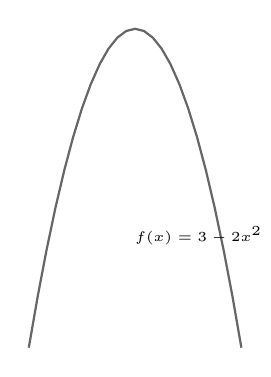
\begin{tikzpicture}[scale=0.9, draw opacity = .6]
	    % abscisa y ordenada
	    \tkzInit[xmax= 3,xmin=-3,ymax=3,ymin=-2]
	    \tiny\tkzLabelXY[opacity=0.6,step=1, orig=false]
	    % label x, f(x)
	    \tkzDrawX[opacity= .6,label=x,right=0.3]
	    \tkzDrawY[opacity= .6,label=f(x),below = -0.6]
	    %dominio y función
	    \draw [domain=-1.5:1.5,thick] plot(\x,{3-2*\x*\x}); 
	    \tkzText[above,opacity=0.6](3.3,3){\tiny $f(x)=3-2x^2$}
	\end{tikzpicture}
    \end{center} 
    \vspace{.5cm}
 
    %--------------------13.
    \item $f(x)=x^2 + 2x - 1$
    \begin{center}
	\begin{tikzpicture}[scale=0.9, draw opacity = .6]
	    % abscisa y ordenada
	    \tkzInit[xmax= 2,xmin=-4,ymax=4,ymin=-2]
	    \tiny\tkzLabelXY[opacity=0.6,step=1, orig=false]
	    % label x, f(x)
	    \tkzDrawX[opacity= .6,label=x,right=0.3]
	    \tkzDrawY[opacity= .6,label=f(x),below = -0.6]
	    %dominio y función
	    \draw [domain=-3.5:1.5,thick] plot(\x,{\x*\x + 2*\x - 1}); 
	    \tkzText[above,opacity=0.6](3.3,3){\tiny $f(x)=x^2 + 2x - 1$}
	\end{tikzpicture}
    \end{center} 
    \vspace{.5cm}

    %--------------------14.
    \item $f(x)=\dfrac{1}{x-1}$
    \begin{center}
	\begin{tikzpicture}[scale=0.9, draw opacity = .6]
	    % abscisa y ordenada
	    \tkzInit[xmax= 3,xmin=-4,ymax=5,ymin=-5]
	    \tiny\tkzLabelXY[opacity=0.6,step=1, orig=false]
	    % label x, f(x)
	    \tkzDrawX[opacity= .6,label=x,right=0.3]
	    \tkzDrawY[opacity= .6,label=f(x),below = -0.6]
	    %dominio y función
	    \draw [domain=-3:0.8,thick] plot(\x,{1/(\x-1)}); 
	    \draw [domain=1.2:3,thick] plot(\x,{1/(\x - 1)}); 
	    \tkzText[above,opacity=0.6](3.3,3){\tiny $f(x)=\dfrac{1}{x-1}$}
	\end{tikzpicture}
    \end{center} 
    \vspace{.5cm}

    %--------------------15.
    \item $f(x)=\sin 2x$
    \begin{center}
	\begin{tikzpicture}[xscale=0.08, draw opacity = .6]
	    % abscisa y ordenada
	    \tkzInit[xmax= 175,xmin=-4,ymax=1,ymin=-1]
	    \tiny\tkzLabelXY[opacity=0.3,step=10, orig=false]
	    % label x, f(x)
	    \tkzDrawX[opacity= .6,label=x,right=0.3]
	    \tkzDrawY[opacity= .6,label=f(x),below = -0.6]
	    %dominio y función
	    \draw [domain=0:175,samples=100] plot(\x, {sin(2*\x)});
	    \tkzText[above,opacity=0.6](3.3,3){\tiny $f(x)=\sin 2x$}
	\end{tikzpicture}
    \end{center} 
    \vspace{.5cm}

    %--------------------16.
    \item $f(x)=\cos 3x$
    \begin{center}
	\begin{tikzpicture}[xscale=0.1, draw opacity = .6]
	    % abscisa y ordenada
	    \tkzInit[xmax= 146,xmin=-4,ymax=1,ymin=-1]
	    \tiny\tkzLabelXY[opacity=0.3,step=10, orig=false]
	    % label x, f(x)
	    \tkzDrawX[opacity= .6,label=x,right=0.3]
	    \tkzDrawY[opacity= .6,label=f(x),below = -0.6]
	    %dominio y función
	    \draw [domain=0:146,samples=100] plot(\x, {cos(3*\x)});
	    \tkzText[above,opacity=0.6](3.3,3){\tiny $f(x)=\cos 3x$}
	\end{tikzpicture}
    \end{center} 
    \vspace{.5cm}

    %--------------------17.
    \item $f(x)=x^2-4x+6$
    \begin{center}
	\begin{tikzpicture}[scale=0.9, draw opacity = .6]
	    % abscisa y ordenada
	    \tkzInit[xmax= 4,xmin=-1,ymax=7,ymin=0]
	    \tiny\tkzLabelXY[opacity=0.6,step=1, orig=false]
	    % label x, f(x)
	    \tkzDrawX[opacity= .6,label=x,right=0.3]
	    \tkzDrawY[opacity= .6,label=f(x),below = -0.6]
	    %dominio y función
	    \draw [domain=-.5:4.5,thick] plot(\x,{\x*\x -4*\x + 6}); 
	    \tkzText[above,opacity=0.6](5,3){\tiny $f(x)=x^2 - 4x + 6$}
	\end{tikzpicture}
    \end{center} 
    \vspace{.5cm}

    %--------------------18.
    \item $f(x)=\dfrac{1}{1-x^2}$\\\\
    \begin{center}
	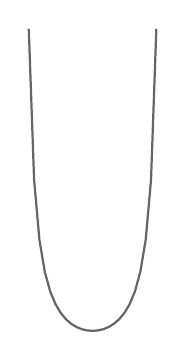
\begin{tikzpicture}[scale=0.9, draw opacity = .6]
	    % abscisa y ordenada
	    \tkzInit[xmax= 2,xmin=-2,ymax=6,ymin=0]
	    \tiny\tkzLabelXY[opacity=0.6,step=1, orig=false]
	    % label x, f(x)
	    \tkzDrawX[opacity= .6,label=x,right=0.3]
	    \tkzDrawY[opacity= .6,label=f(x),below = -0.6]
	    %dominio y función
	    \draw [domain=-.9:.9,thick] plot(\x,{1/(1-\x*\x)}); 
	    \tkzText[above,opacity=0.6](4,3){\tiny $f(x)=x^2 - 4x + 6$}
	\end{tikzpicture}
    \end{center} 
    \vspace{.5cm}

    %--------------------19.
    \item $f(x)=\sin\left(x + \dfrac{\pi}{4} \right)$\\\\
    \begin{center}
	\begin{tikzpicture}[xscale=0.08, draw opacity = .6]
	    % abscisa y ordenada
	    \tkzInit[xmax= 175,xmin=-4,ymax=1,ymin=-1]
	    \tiny\tkzLabelXY[opacity=0.3,step=10, orig=false]
	    % label x, f(x)
	    \tkzDrawX[opacity= .6,label=x,right=0.3]
	    \tkzDrawY[opacity= .6,label=f(x),below = -0.6]
	    %dominio y función
	    \draw [domain=0:175,samples=100] plot(\x, {sin(\x + (pi/4))});
	    \tkzText[above,opacity=0.6](3.3,3){\tiny $f(x)=\sin\left(x + \dfrac{\pi}{4} \right)$}
	\end{tikzpicture}
    \end{center} 
    \vspace{.5cm}

    %--------------------20.
    \item $f(x)=\cos \left( x - \dfrac{\pi}{3} \right)$\\\\
    \begin{center}
	\begin{tikzpicture}[xscale=0.08, draw opacity = .6]
	    % abscisa y ordenada
	    \tkzInit[xmax= 175,xmin=-4,ymax=1,ymin=-1]
	    \tiny\tkzLabelXY[opacity=0.3,step=10, orig=false]
	    % label x, f(x)
	    \tkzDrawX[opacity= .6,label=x,right=0.3]
	    \tkzDrawY[opacity= .6,label=f(x),below = -0.6]
	    %dominio y función
	    \draw [domain=0:175,samples=100] plot(\x, {cos(\x - (pi/3))});
	    \tkzText[above,opacity=0.6](3.3,3){\tiny $f(x)=\cos \left( x - \dfrac{\pi}{3} \right)$}
	\end{tikzpicture}
    \end{center} 
    \vspace{.5cm}

    %--------------------21.
    \item $f(x) = \tan \dfrac{1}{2} x$\\\\
    \begin{center}
	\begin{tikzpicture}[xscale=0.08, draw opacity = .6]
	    % abscisa y ordenada
	    \tkzInit[xmax= 75,xmin=-4,ymax=1,ymin=-1]
	    \tiny\tkzLabelXY[opacity=0.3,step=10, orig=false]
	    % label x, f(x)
	    \tkzDrawX[opacity= .6,label=x,right=0.3]
	    \tkzDrawY[opacity= .6,label=f(x),below = -0.6]
	    %dominio y función
	    \draw [domain=0:70,samples=100] plot(\x, {tan(\x - (pi/3))});
	    \tkzText[above,opacity=0.6](3.3,3){\tiny $f(x)=\tan \dfrac{1}{2} x$}
	\end{tikzpicture}
    \end{center} 
    \vspace{.5cm}


\end{enumerate}
